\section{Wrap-up {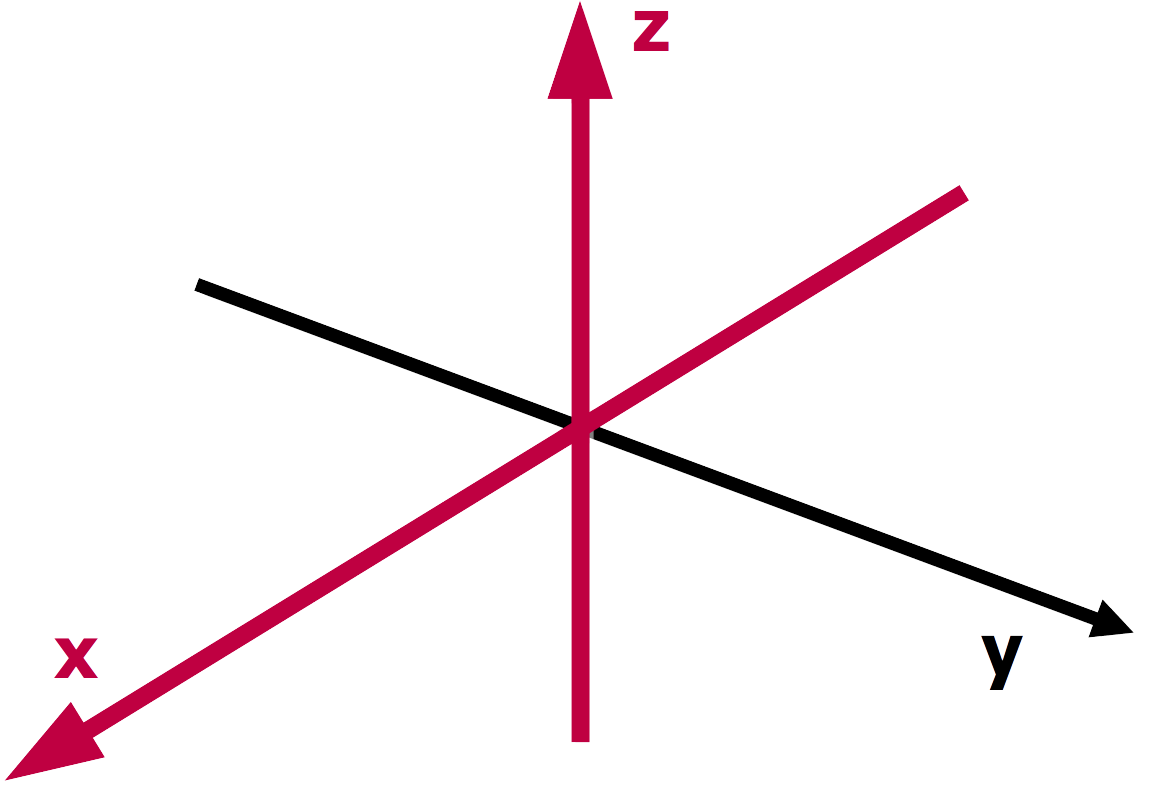
\includegraphics[height=15pt]{connectivity-xz-small}}}

{
\usebackgroundtemplate{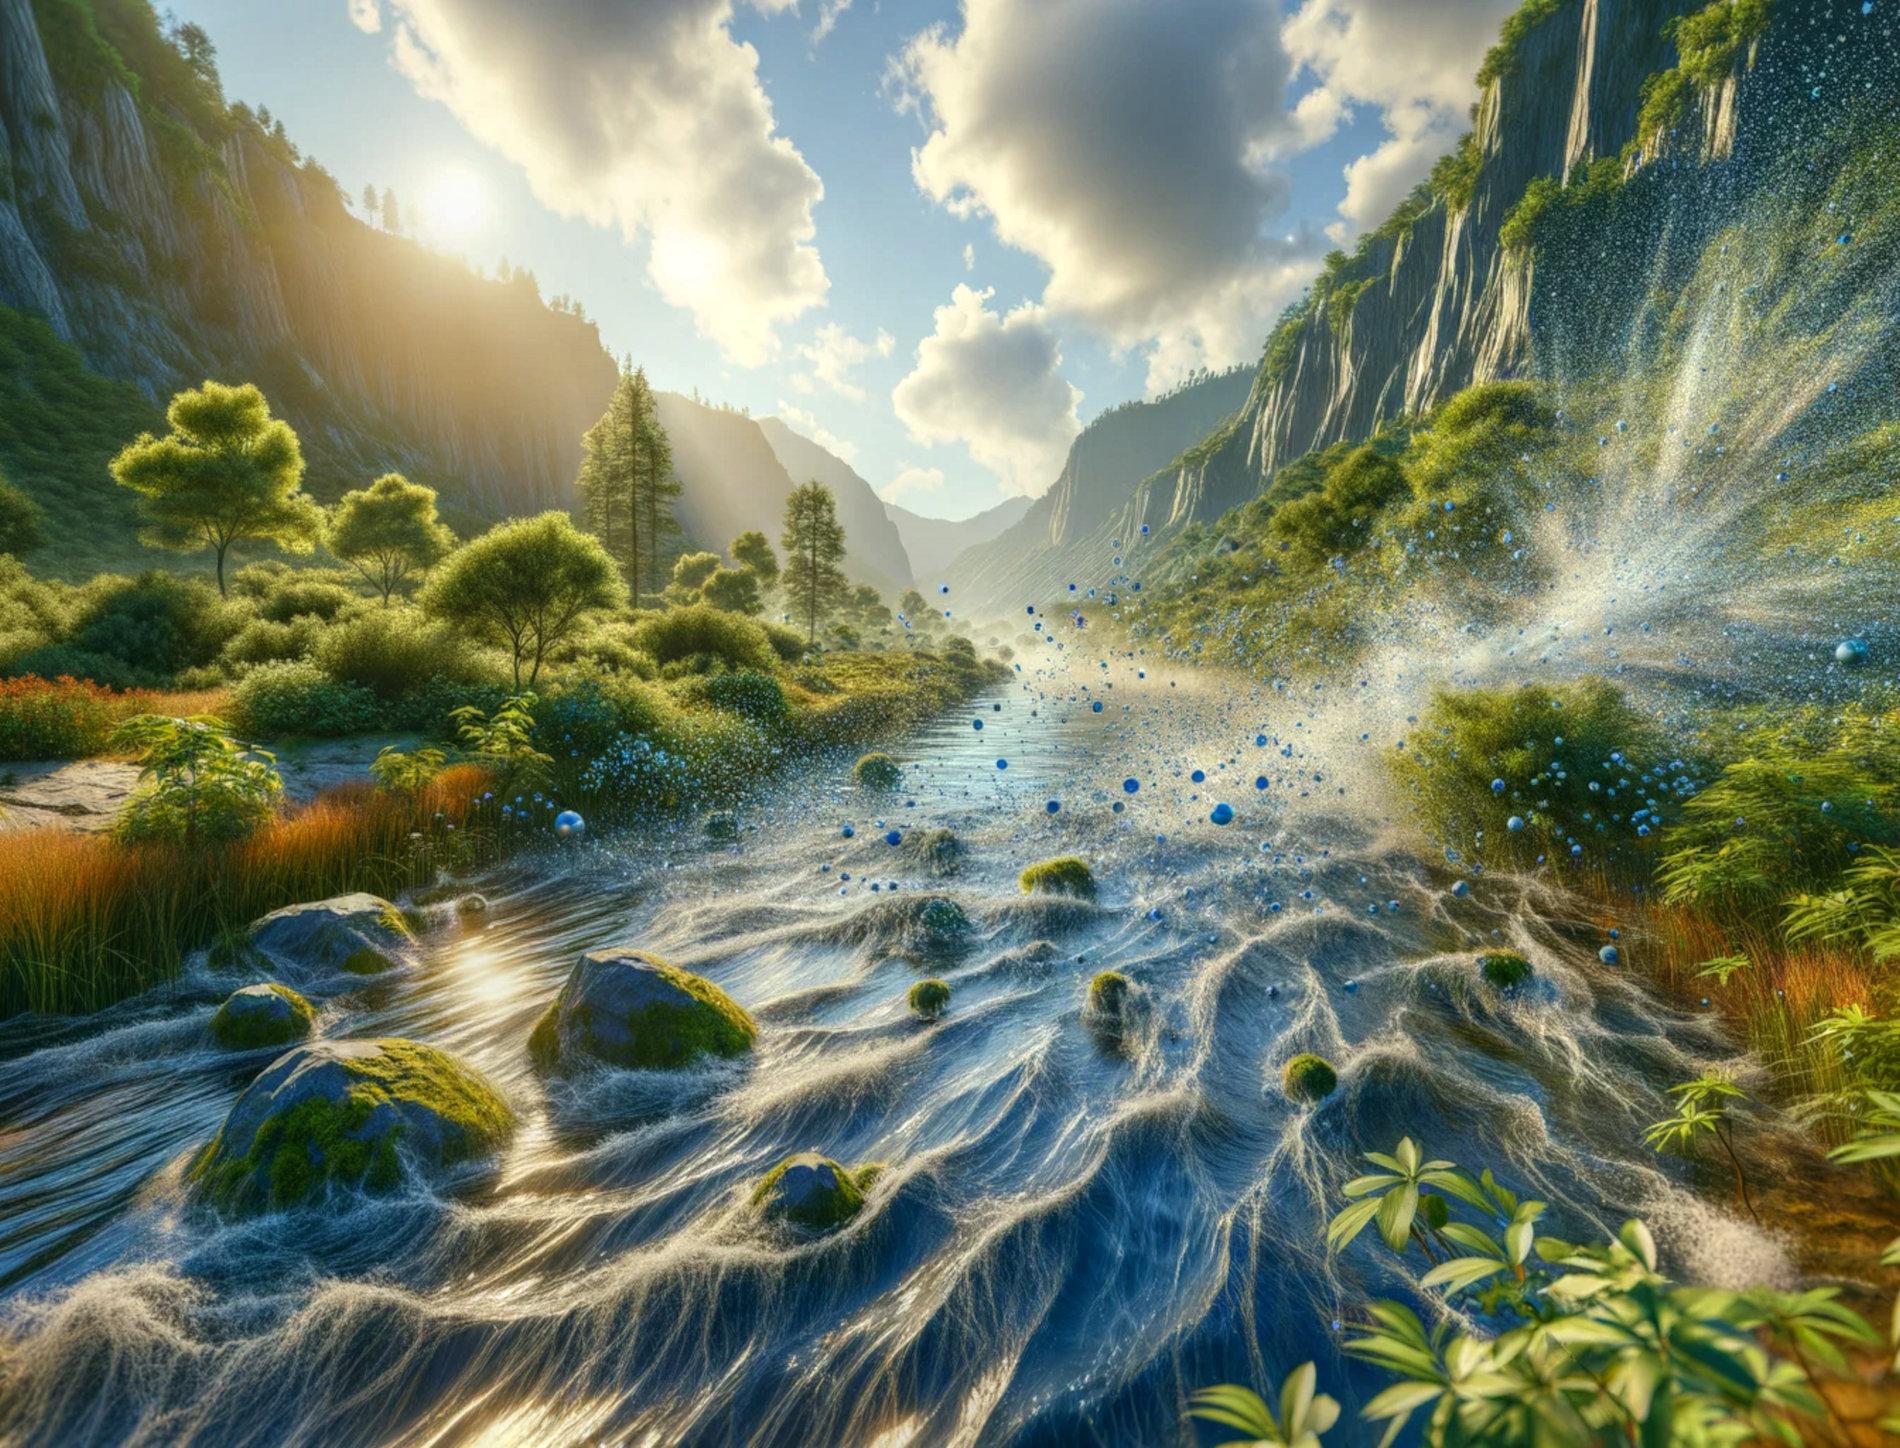
\includegraphics[width=\paperwidth]{final-background43.jpg}}%
\begin{frame}[plain]{}{\secname}
	\vspace{2.cm}
		\begin{tcolorbox}[colbacktitle=hellblau!80!black, colback=hellblau!10!white, fonttitle=\bfseries, standard jigsaw,colframe=blue_light, bottom=0mm, middle=0mm, boxsep=0.2mm, opacityframe=0.5, opacityfill=0.65, opacitybacktitle=0.75, title filled, title={\faGraduationCap\ Conclusions}, size=fbox]
			\vspace{0.25cm}
			\begin{itemize}			
				\item[\faChainBroken] Dams block primarily coarse sediment \& let pass very fine sediment\\
				$\rightarrow$ Downstream of dams: coarse sediment-hungry rivers only get fine sediment\\
				$\rightarrow$ Vertical disconnection (riverbed clogging) \& lateral disconnection \vspace{0.1cm}
				\item[\faLightbulbO] Numerical modeling provides predictive guidance for local actions, but calibration is challenging
				\item[\faLightbulbO] Local actions: improved sediment continuity in mountain rivers \& large wood placement
			\end{itemize}
			\vspace{0.1cm}
			\movie[externalviewer]{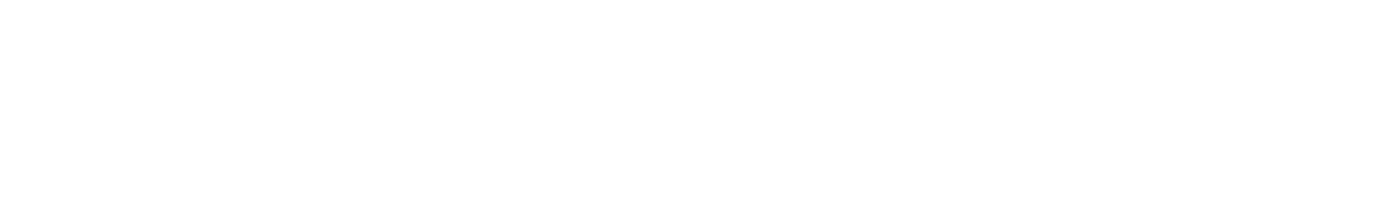
\includegraphics[width=0.6\textwidth,keepaspectratio]{videos/blank-wide.png}}{videos/ue-fishpass-clip.mp4}
		\end{tcolorbox}
		\smallskip
\end{frame}
}

